\documentclass[titlepage,11pt,twoside]{article}



\usepackage[dvips]{graphicx}

\usepackage[myheadings]{fullpage}
\usepackage{pmetrika}
\usepackage{pmbib}
\usepackage{color}
\usepackage{mathtools}
\usepackage{amssymb}
\usepackage{hyperref}
\usepackage{natbib}
\usepackage{multirow}
%\usepackage[backend=biber,natbib=true, style=authoryear-comp]{biblatex}





%\usepackage{submit}

\newcommand{\bfU}{\mbox{\boldmath$\mathsf{U}$}}
\newcommand{\bfu}{\mbox{\boldmath$\mathsf{u}$}}
\newcommand{\hl}[1]{\textcolor{magenta}{#1}}
\newcommand{\RR}{\mathbb{R}}
\DeclareMathOperator*{\V}{V}
\newcommand{\argmax}{\text{argmax}}
\newcommand{\R}[1]{\texttt{#1}}
\newcommand{\acos}{\text{arccos}}


%\begin{figure}[h]
%\centerline{\includegraphics{figure03.eps}}
%\caption{Projection of item discrimination vectors onto $V_{\theta_T}$ hyperplance for a six item three-dimensional approximate sample structure.}
%\end{figure}


%\raggedbottom
\flushbottom


%\firstpage{1}
%\setcounter{lastpage}{999}
\setcounter{secnumdepth}{3}

\begin{document}

\linespacing{1}

%\title{Something that is not PCADSC}
%\title{Structure comparison for multivariate data by\ldots / with application to \ldots}
\title{Exploratory data structure comparisons: Three new tools based on Principal Component Analysis}

\author{Anne H. Petersen, Bo Markussen, Karl Bang Christensen}

\affil{University of Copenhagen}


\vspace{\fill}




\linespacing{1}

%\RepeatTitle{Psychometrics: From Practice to Theory and Back}

\begin{center}\vskip3pt


\vspace{32pt}

Abstract\vskip3pt

\end{center}


\begin{abstract}
abstract...
\begin{keywords}
keywords...
\end{keywords}
\end{abstract}

\vspace{\fill}\newpage

\section{Introduction}
\label{sec:introduction}

Classical statistical methodology is aimed at analyzing data from designed experiments and historically, statistical analyses have been done by researchers who knew the design and origin story of the data set well. However, the origin stories of data sets have changed over time and today a lot of data is accumulated without a specific purpose in mind. This is due to vast amounts of data being registered online and to a trend towards more open source research. The latter phenomenon in particular poses new challenges wrt. data quality assessment. When data are collected and made public without a specific end-point in mind, how do we ensure that differences in, say, choice measurement instruments, mode of administration, or sampling frame do not cause the data to be effectively divided into subsets that are simply not comparable?

Surveys often use mixed modes of administration, e.g. mail and telephone, and while this can improve response rates, the mode of administration can affect results \cite{Brambilla1987,McHorney1994} and differences in response behavior can lead to biased results. Powers, Mishra and Young \citeyearpar{Powers2005} report effects of mode of administration on changes in mental health scores that are of a magnitude that is considered to be clinically meaningful.

The rapid growth of web surveys, due to low cost, timeliness, and other factors, generate large data sources that lack a sampling frame of the general population. However, it can be problematic to combine online panels (pre-recruited profiled pools of respondents) with intercept samples (a pool of respondents obtained through banners, ads, or promotions) \cite{Liu2016}.

Sophisticated methods for addressing this question are available when we are willing to assume a statistical model, but when these models are taken away, a remarkable void of methods is left behind. What is needed is a procedure that compares differences in overall data structures in two (or more) subsets of a dataset without assuming neither directional nor hierarchical relationships between the variables. We propose a suite of three new tools for this task, which we will refer to collectively as Principal Component Analysis-based Data Structure Comparisons (PCADSC). These methods employ the principal component decomposition of the empirical covariance matrix performed on two subsets of a dataset in order to create intuitive visualizations of data structure differences. Software for using these tools is available in an \texttt{R}-package. \hl{how to refer to our package?}


This manuscript is structured as follows: First, in Section \ref{sec:stateoftheart}, we present the data structure comparison problem in more detail and discuss what statistical methods are already available for solving similar challenges. Next, in Section \ref{sec:pcadscintro}, we move on to a description of the PCADSC procedures, including a brief introduction to principal component analysis (PCA) in general. In Section \ref{sec:dataexample}, we present a worked data example using open source, online available data on psychological well-being in three European countries. More specifically, we compare data from Denmark, which has been repeatedly been rewarded "happiest country in the world", with data from Bulgaria and Sweden, respectively, to investigate whether or not psychological well-being - and thus happiness - is really a concept that is universal beyond country borders, or if such rankings of happiness are inherently meaningless. At last, we discuss limitations and merits of the PCADSC tools in Section \ref{sec:discussion}. 



\section{Something about state of the art}
\label{sec:stateoftheart}
\subsection{\hl{More detailed description of the type of problem we wish to address}}
\hl{
\begin{itemize}
\item Two subsets of a dataset, i.e. to datasets with the same variables, but different observations
\item Wish to compare structures without specifying a model or even any variables of interest
\item The most central example is the question of whether the two subsets can readily be combined in a (unknown) data analysis, or if the subset-inducing variable actually implies heterogeneity across the subset division
	\begin{itemize}
		\item Examples: Large scale open source datasets such as the PISA data and ESS (European Social Survey) data and ...(?). In these datasets, the data producers are very far away from the majority of the data analysts. Therefore, problem-specific recommendations about potential instrument-induced challenges in the datasets are not available for the data analysts. How can data producers ensure that this will not be an issue, at least not related to known data gathering differences?
		\item Other examples?
		\item Perhaps a description of what happens if we are to combine the two subsets of the datasets without taking a e.g. an instrument-effect into account. When will it cause problems (maybe: causal graph style?)?
		\item Mention somewhere: We want a solution that is largely independent of the sizes of the two subsets of data. Thereby, a lot of methods that compare each subset to the full dataset in some sense are excluded.
	\end{itemize}
\end{itemize}
}

\subsection{\hl{Describe existing methods used to solve similar questions or parts of the question we are addressing}}
\hl{
\begin{itemize}
\item The simplest case: variable-by-variable tests in distributional differences
	\begin{itemize}
		\item Simple, but scales poorly
		\item Only relates to marginal differences and not to the interplay between variables
	\end{itemize}
\item Karl's papers?
\item Anne's papers: IRT-based methods for surveys
	\begin{itemize}
		\item Moves beyond the marginal approach, but needs a model pre-specified
		\item Thus, it is not a general data structure comparison method, but rather a fitted-model comparison method. It addresses the interplay between the model and the data, not the data alone. This is fundamentally a different (though related) question.
	\end{itemize}
\end{itemize}
}


\section{PCADSC - description of the method}
\label{sec:pcadscintro}
\hl{Description from Anne's master's thesis. Rewrite.}

As mentioned above, the purpose of PCADSC is comparing overall data structures in two or more subsets of a dataset. But before we can get further into describing this procedure, we must first define what exactly is meant by "overall structure". One such definition is the structure of the covariance matrix of the dataset. If we assume all variables in the dataset to be jointly normal with zero means, the covariance matrix is a sufficient statistic for describing the simultaneous distribution of all the variables. This gives it a very nice interpretation as a measure of the overall structure. If we do not accept the normality assumption, pairwise correlations and variable variances are still interesting quantities that say something about the interrelations between the variables, at least in terms of linear relationships. All in all, the empirical covariance matrix is a reasonable place to start looking for differences in "overall data structures".

Though the idea sounds appealing, it is quite difficult to assess similarity of matrices, and moreover, this becomes increasingly difficult for large numbers of variables and thus high dimensional covariance matrices. There is simply too much information to consider at once.

However, by 
%clever 
use of linear algebra, we can construct a decomposition of the covariance matrix that makes it easier to gain an overview of the data. We propose a new method based on principal component analysis that seems to be able to identify differences in datasets based on intuitive, visual inspections. We refer to this method as principal component analysis-based data structure comparison (PCADSC) and we present the procedure below. But first, we give a minimal introduction to principal component analysis in general with reference to Koch (2014).


\subsection{Principal component analysis}

Consider $n$ observations $x_1,\dotsc,x_n \in \RR^d$ of $d$ variables, let $\bar{x} = \frac{1}{n} \sum_{i=1}^n x_n$ denote their average\hl{(s?)} and let $S = \frac{1}{n-1} \sum_{i=1}^n (x_i-\bar{x}) (x_i-\bar{x})^\top \in \RR^{d \times d}$ denote the empirical covariance \hl{Is $\bar{x} \in \RR^d$ with $\bar{x} = (\bar{x_1}, ..., \bar{x_d})^T$?}. Suppose that we want to describe the observations by $q$ numbers instead of the original $d$ numbers. The associated \emph{rank-q-reconstruction error} is defined as the minimal squared error that is achievable by linear subspaces $K_q \subset \RR^d$ of dimension $q < d$, that is
\begin{equation*}
\min_{K_q} \sum_{i=1}^n \min_{z \in K_q} \lVert x_i - \bar{x} - z \rVert^2 =
\min_{K_q} \sum_{i=1}^n \lVert x_i - \bar{x} - \text{proj}_{K_q}(x_i - \bar{x}) \rVert^2.
\end{equation*}
\emph{Principal component analysis} (PCA) ensures the existence of a subspace $\hat{K}_q \subset \RR^d$ that attains this minimum, and it provides an explicit description of $\hat{K}_q$ and the rank-q-reconstruction error. Thus, let $S = U \Lambda U^\top$ be the eigenvalue decomposition of $S$. Here $\Lambda \in \RR^d$ is the diagonal matrix with the eigenvectors $\lambda_1 \ge \dotsm \ge \lambda_d \ge 0$ in the diagonal, and $U \in \RR^d$ is the orthogonal matrix with the associated eigenvectors $\eta_1,\dotsc,\eta_d \in \RR^d$ in the columns. The eigenvalues are uniquely defined, and the eigenvectors are uniquely defined up to a change of sign whenever the eigenvalues are different. If some of the eigenvalues are identical, e.g.\ $\lambda_i=\lambda_{i+1}=\dotsm=\lambda_j$, then the associated eigenvectors $\eta_i,\eta_{i+1},\dotsc,\eta_j$ are uniquely defined up to a common rotation. In practice this only happens if $n < d$, in which case the last $d-n$ eigenvalues will be zero \hl{Anne: What about covariance matrices that are not of full rank (e.g. because of colinearity)? Won't we find eigenvalue multiplicities $> 1$ here as well?}. It is a result from linear algebra that the rank-q-reconstruction error for $q < d$ is achieved for
\begin{equation*}
\hat{K}_q = \text{span}\{\eta_1,\dotsc,\eta_q\}
\end{equation*}
and equals $\sum_{j=q+1}^d \lambda_j$. The eigenvectors $\eta_j \in \RR^d$ are called \emph{loadings}, and the eigenvalues $\lambda_j \ge 0$ may be understood as \emph{variation components}. The projections $\eta_j^\top (x_i - \bar{x})$ of the observations onto the loadings are called \emph{scores}. The $j$th loading can also be found iteratively as the unit vector $u \in \RR^d$ orthogonal to $\hat{K}_{j-1}$, where the initial subspace is defined as $\hat{K}_0 = \{0\}$, that maximizes the variation of the associated scores:
\begin{align*}
\eta_j &= \argmax_{u \in \RR^d\colon u \perp \hat{K}_{j-1}} \sum_{i=1}^n \lVert u^\top (x_i - \bar{x}) \rVert^2, &
\lambda_j &= \frac{1}{n-1} \sum_{i=1}^n \lVert \eta_j^\top (x_i - \bar{x}) \rVert^2.
\end{align*}
\hl{Anne: Should we maybe assume standardized $x$s here also? I feel like it is part of the PCA algorithm and subtracting the mean in the above seems off for that reason. Also: Something is wrong with the dimensions here. $u$ is $d \times 1$, $x_i$ is $d \times 1$(?) - how do we get $\eta_j$ to also be $d \times 1$?} It is worth emphasizing that the greedy approach of successively adding the next direction $\eta_j$ explaining most of the remaining variation, also gives the sequence $\hat{K}_q = \hat{K}_{q-1} \oplus \text{span} \{\eta_q\}$ of subspaces minimizing the rank-q-reconstruction error. This strong interpretation of PCA, which is often overlooked in the literature, means that the sequence of loadings $\eta_j$ and their associated variation components $\lambda_j$ yield a simultaneous description of the structure of the data set for all approximating dimensions $q$. This implies that the loadings and variation components can be used to investigate the structure of the data set without the need to decide on an approximating dimension $q$.


%Principal component analysis (PCA) allows us to decompose a data matrix consisting of $n$ observations of $d$ variables into $d$ orthogonal vectors of length $d$. This is in itself not very impressive nor useful. But PCA does not result in just any basis of the data matrix. The basis chosen using PCA has the very favorable property that each vector is chosen such that they maximize the accumulated explained variance. These vectors are usually denoted \textit{principal component scores} or simply \textit{principal components} and they are constructed as linear combinations of the variables in the dataset (or, equivalently, as projections of the data matrix). The coefficients of each variable in these projections are denoted \textit{loadings}. Let $S \in \RR^{d \times d}$ denote the empirical covariance matrix and let $X \in \RR^{n \times d}$ denote our observed data matrix. $d$ is the number of variables while $n$ is the number of observations. The deconstruction procedure then goes as follows:
%\begin{enumerate}
%\item The vector of loadings corresponding to the first principal component, $\eta_1 \in \RR^d$, is chosen such that the component explains as much variance as possible. More precisely, for any unit vector $u \in \RR^d$ we find that $\V(u^T X^T)$ is maximized when $u = \eta_1$. Let $\lambda_1 = \V(\eta_1^T X^T)$.
%\item The second vector of loadings is then chosen as $\eta_2 = \argmax_{u: \, u \perp \eta_1} \V(u^T X^T)$ and we again define $\lambda_2 := \V(\eta_2 X)$.
%\item The third vector of loadings is $\eta_3 = \argmax_{u: \, u \perp \{\eta_1, \eta_2\}} \V(u^T X^T)$ and $\lambda_3 :=  \V(\eta_3^T X^T)$ \\
%\vdots
%\item[\refstepcounter{enumi} $d$.] The $d$th vector of loadings is $\eta_d = \argmax_{u: \, u \perp \{\eta_1, ..., \eta_{d-1}\}} \V(u^T X^T)$ and $\lambda_d = V(\eta_d^T X^T)$.
%\end{enumerate}
%The $\eta_i$s and $\lambda_i$s are determined uniquely (up to scaling) and they are given as the eigenvectors and eigenvalues of $S$, respectively. Moreover, we find that $X = \sum_{i=1}^d \eta_j \eta_j^T X$, so the procedure is really just a clever choice of rotation of the data, such that it is split up into vectors that are ordered by their variances, or more precisely, their variance contributions. We define the contribution to the total variance of the $k$th principal component as $\frac{\lambda_k}{tr(S)}$ and please note that, due to the properties of eigenvalue decomposition, $tr(S) = \sum_{i=1}^d \lambda_i$, which is the sum of the variances of the variables in the dataset.
%
% In this introduction, we have assumed full rank of the covariance matrix $S$ for simplicity, but it should be noted that this assumption is in no way needed for the results to hold.

\subsection{PCA-based data structure comparisons}
Above, we promised a method for intuitive, visual inspection of data structure similarities, but as of now, all intuition might have been lost in technicalities. The main point we want to emphasize from PCA is that whereas the scores describe the observations, the variation components and the accompanying loadings describe the usage of the variables. If two different datasets with the same variables, but different samples of observations, have similar loading patterns, then the variables appear to be measuring the same underlying quantities in both data situations. This can be the case while the two sets of scores could be arbitrarily different, which e.g.\ could happen if the two datasets were taken from two different populations of subjects. On the other hand, if the loading patterns are different in the two datasets, then this indicates that the variables are used differently in the two data situations, and hence it would be criticizable to use these variables for comparisons across the two datasets.

%Specifically, we can interpret the loadings as weights that determine the relative influence of each variable in each principal component.

%the two data sets will agree on which variables explain the most variance and also how this variance is explained.  Looking at the PCA loadings and the cumulative explained variance thus provides a straightforward non-parametric graphical approach for assessing similarity between two datasets.

In this paper we propose three diagnostic plots for comparing the loading patterns in two datasets $x_{11},\dotsc,x_{1 n_1} \in \RR^d$ and $x_{21},\dotsc,x_{2 n_2} \in \RR^d$ in the same $d$ variables. The construction of these plots, which we call \emph{CumEigenPlot}, \emph{HairPlot} and \emph{PancakePlot}, proceeds in the following steps:
\begin{enumerate}
\item Standardized the observations $x_{i1},\dotsc,x_{i n_i}$ to have zero mean and unit standard deviation separately for each of the $d$ variables within each datasets. Let $\tilde{x}_{ij} \in \RR^d$ for $i=1,2$ and $j=1,\dotsc,n_i$ be the standardized observations, and form the principal component analysis
\begin{equation*}
S_i = \frac{1}{n_i-1} \sum_{j=1}^{n_i} \tilde{x}_{ij} \tilde{x}_{ij}^\top = \sum_{k=1}^d \lambda_{ik} \eta_{ik} \eta_{ik}^\top \quad \text{for $i=1,2$.} 
\end{equation*}
\item Combine the standardized datasets into a joint dataset $\tilde{x}_1,\dotsc,\tilde{x}_n \in \RR^d$ with $n=n_1+n_2$ observations, standardize this dataset, and form the principal component analysis
\begin{equation*}
S = \frac{1}{n-2} \sum_{j=1}^n \tilde{x}_j \tilde{x}_j^\top = \sum_{k=1}^d \lambda_k \eta_k \eta_k^\top.
\end{equation*}
\item Make the diagnostic plot of interest. Details of the plots will be described below.
\item To investigate the sample variation randomly reallocate the combined and standardized dataset formed in step 2 to two datasets of $n_1$ and $n_2$ observations, respectively, and redo step 1 and 3. This is done several times, e.g.\ 10000 times, and compared to the plot for the original allocation.
\end{enumerate} 

Before describing the details of the  \emph{CumEigenPlot}, \emph{HairPlot} and \emph{PancakePlot} we make some general remarks. First, it should be noted that PCA is sensitive to scaling, as the procedure deconstructs the covariance matrix in components according to the most explained variance. This implies that if a variable has a very large sample variance (possibly because of its scale), this variable will be always be deemed highly influential, no matter the structure of the data. Therefore, the variables should always be scaled prior to performing PCA. Note that the covariance matrix for the standardized variables is the same as the correlation matrix for the original variables, so this simply corresponds to performing data structural comparisons of the correlation matrices rather than the covariance matrices. \hl{Do we still need more about this topic? Then we can add something like:
\begin{itemize}
\item Following the greedy interpretation of PCA, we know that the first eigenvector is chosen as
$$\eta_1 = \argmax_{u \in \RR^d} \sum_{i=1}^n \lVert u^\top (x_i - \bar{x}) \rVert^2  = \text{argmax}_{u \in \RR^d} \tilde{\V}(u^T X^T) $$
\item Now, imagine that $\V(x_1) >> \V(x_j)$ for all $j \in 2, ..., d$. Note that $(1, 0, ..., 0) X^T = x_i$. Then, clearly a vector $u$ that only picks out the first variable from the data matrix $X$, namely $u^T = (1, 0, ..., 0)$ will allow us to only look at the variance of $x_1$, which is very large. This has nothing to do with the interplay between variables, as the phenomenon will disappear if we scale $x_1$
\item A more formal explanation could come from this kind of intuition, if needed.
\end{itemize}
}
The standardization makes the variables comparable on the same scale, i.e.\ units of standard deviation, and it implies that the diagonal elements of $S$, $S_1$, and $S_2$ all equals 1. This also holds for the reallocated datasets, and in particular we have $\sum_{k=1}^d \lambda_k = \sum_{k=1}^d \lambda_{1k} = \sum_{k=1}^d \lambda_{2k} =  d$. The random reallocations in step 4 provide resamples under the null hypothesis that the two sample populations have the same structure in the $d$ variables, except that the two populations are allowed to have the own standard deviations for each of the variables. This exception is induced by the initial step 1, which performs a standardization within the two datasets before they are combined in step 2. These resamples can be used for a visualization of the sample variation, and if a test statistic can be defined in step 3, then a $p$-value for the null hypothesis may be computed. Such $p$-values are know as permutation tests for Goodness-of-Fit (\hl{reference?}).

%In order to describe these plots we consider two different datasets in the same $d$ variables and with $n_1$ and $n_2$ observations, respectively. For dataset $i=1,2$ let $S_i \in \RR^{d \times d}$ be the empirical correlation matrix \hl{(find a way to introduce the empirial correlation matrix instead)}, and let $\lambda_{i1} \ge \dotsm \ge \lambda_{id} \ge 0 $ and $\eta_{i1},\dotsc,\eta_{id} \in \RR^{d}$ be the corresponding variation components and loadings. The correlation matrices correspond to the covariance matrices for the variables after these have been standardized to unit standard deviation separately within the two datasets. Similarly, let $S \in \RR^{d \times d}$ be the empirical correlation matrix for the combined dataset with $n_1+n_2$ observations, and let $\lambda_1 \ge \dotsm \ge \lambda_d \ge 0$ and $\eta_1,\dotsc,\eta_d \in \RR^d$ be the corresponding variation components and loadings.

\hl{To do: Something about what to do if not all variables are numerical. Anne: Maybe leave this for the discussion?
%Using correlation matrices is not the same as assuming standadized variables; there is a difference in the permutations.
}

\medskip

\subsubsection{Description of the \emph{CumEigenPlot}}
 This plot compares the variation components. 
%If these are the same in the two sample populations, then the best estimate for the variation components are $\lambda_1 \ge \dotsm \ge \lambda_d \ge 0$ found in the combined dataset. And we would expect $\lambda_{i1} \ge \dotsm \ge \lambda_{id} \ge 0$ for $i=1,2$ to be alike excepts sample variation. 
In order to investigate whether the same proportion of the total variation can be described by the same number of principal components in the two datasets we plot a piecewise linear curve connecting the points
\begin{align*}
(0,0), &&
(\lambda_1,\lambda_{11}-\lambda_{12}), &&
(\lambda_1 + \lambda_2,\lambda_{11}+\lambda_{12}-\lambda_{21}-\lambda_{22}), &&
\ldots, &&
\bigg( \sum_{j=1}^d \lambda_j, \sum_{j=1}^d \lambda_{1j} - \sum_{j=1}^d \lambda_{2j} \bigg).
\end{align*}
This may be seen as a cumulated Bland-Altman plot for the variation components (\hl{reference to cumulated residuals and to Bland-Altman}). Note that due to the standardization the last point will be equal to $(d,0)$. Thus, this curve will begin and end at the x-axis. And the larger excursions it makes away from the x-axis the less alike the cumulated variation components for the two datasets are. \hl{Is this an informative x-axis? Should we maybe consider scaling it?}

In step 3 we have implemented both the \emph{Kolmogorov-Smirnov} and the \emph{Cram\'er-von Mises} test statistics given by
\begin{align*}
\text{KS} &= \max_{k=1,\dotsc,d} \bigg\lvert \sum_{j=1}^k \lambda_{1j} - \sum_{j=1}^k \lambda_{2j} \bigg\rvert, &
\text{CvM} &= \sum_{k=1}^{d-1} \frac{\lambda_k + \lambda_{k+1}}{2} \bigg( \sum_{j=1}^k \lambda_{1j} - \sum_{j=1}^k \lambda_{2j} \bigg)^2.
\end{align*}
\hl{Maybe more here on what the null hypothesis and range of these test statistics are?} 
From the random reallocations in step 4 we get $p$-values for the Kolmogorov-Smirnov and the Cram\'er-von Mises Goodness-of-Fit tests. Step 4 is also used to visualize the sampling variation in a display, where we plot the observed curve together with 20 of the resampled curves as well as a shaded region visualizing pointwise 95 \% coverage intervals. If the observed curve is very different from the resampled curves or if it is substantially outside the shaded region, then this also indicates differences between the two datasets.

%Whether the excursions in the observed curve are large or within the range of sample variation can be quantified by a permutation test. The idea is that we randomly reallocate the $n_1+n_2$ observations in the combined dataset to two datasets with $n_1$ and $n_2$ observations, respectively, and then repeat the procedure described above. The random reallocation by construction ensures that the two resampled datasets are alike except their sample size and sampling variation. In the \emph{CumEigenPlot} we make 1000 independent random reallocations, and plot  P-values for the null hypothesis that the variation components are the same are easily provided for any appropriate test statistic by the resampling procedure as well. 

\bigskip

\subsubsection{Description of the \emph{HairPlot}} 
This plot simultaneously compares the variation components and the loadings. Let $\lambda_{\max} = \max\{ \lambda_{11}, \lambda_{21} \}$ be the largest variation component for the two datasets. The empirical correlation matrix $S_1$ for the first dataset has the following orthogonal decomposition in the coordinate system of the second dataset
%\begin{equation*}
%S_1 = \sum_{k=1}^d \lambda_{1k} \eta_{1k} \eta_{1k}^\top
%= \lambda_{\max} \sum_{k=1}^d
%\Bigg( \sum_{j=1}^d \sqrt{\frac{\lambda_{1k}}{\lambda_{\max}}} (\eta_{1k} \eta_{2j}^\top) \eta_{2j} \Bigg)
%\Bigg( \sum_{j=1}^d \sqrt{\frac{\lambda_{1k}}{\lambda_{\max}}} (\eta_{1k} \eta_{2j}^\top) \eta_{2j} \Bigg)^\top,
%\end{equation*}
\begin{equation*}
S_1 = \sum_{k=1}^d \lambda_{1k} \eta_{1k} \eta_{1k}^\top
= \lambda_{\max} \sum_{k=1}^d
\Bigg( \sum_{j=1}^d \sqrt{\frac{\lambda_{1k}}{\lambda_{\max}}} \eta_{2j} (\eta_{2j}^\top \eta_{1k}) \Bigg)
\Bigg( \sum_{j=1}^d \sqrt{\frac{\lambda_{1k}}{\lambda_{\max}}} \eta_{2j} (\eta_{2j}^\top \eta_{1k}) \Bigg)^\top,
\end{equation*}
and we have a similar decomposition of $S_2$ in the coordinate system of the first dataset \hl{Anne: it was not completely clear to me what this meant the first xx times I read it - expand?}. We propose to visualize these two decompositions in a $d \times d$ grid display. In the $j$th row and $k$th column of this display we plot two arrows based at the lower left corner of the grid cell. The first arrow has length $\mu_{jk}$ and angle $\theta_{jk}/2$ anticlockwise from the diagonal, and the second arrow has length $\nu_{jk}$ and angle $\theta_{jk}/2$ clockwise from the diagonal. To facilitate the following description we will refer to the arrows drawn anticlockwise as the blue arrows, and the arrows drawn clockwise as the red arrows. The lengths $\mu_{jk}$ and $\nu_{jk}$ and the angle $\theta_{kj}$ are given by
\begin{align*}
\mu_{jk} &= \sqrt{\frac{\lambda_{1k}}{\lambda_{\max}}} \lvert \eta_{1k}^\top \eta_{2j} \rvert, &
\nu_{jk} &= \sqrt{\frac{\lambda_{2j}}{\lambda_{\max}}} \lvert \eta_{2j}^\top \eta_{1k} \rvert, &
\theta_{jk} &= \acos(\lvert \eta_{1k}^\top \eta_{2j} \rvert).
\end{align*}
\hl{Maybe emphasize inner product/angle-interpretation here?}
The absolute value of the projection $\eta_{1k} \eta_{2j}^\top$ is inserted due to the indeterminacy of the direction of loading vectors. This indeterminacy implies that the angle between loadings from the two datasets always can be chosen to be in the interval $[0,\pi/2]$, and hence the decomposition of $S_1$ and $S_2$ can be visualized in a joint plot by dividing the angles by two and using anticlockwise and clockwise shifts from the diagonal. Furthermore, the scaling of the lengths by $\lambda_{\max}$ is made so that the longest arrow has at most unit length.

In the \emph{HairPlot} the blue arrows in the $k$th column of the grid display visualize the decomposition of the $k$th principal component for the first dataset in the coordinate system of the second dataset. Similarly, the red arrows in the $j$th row visualize the decomposition of the $j$th principal components for the second dataset in the coordinate system of the first dataset. \hl{Can we expand on this in a non-technical way?} If the structures of the two datasets are identical, then we will have coinciding blue and red arrows along the diagonal in the grid display, and nothing else as arrows in the off-diagonal cells would have zero length. Differences in the variation components are visualized as differences in the lengths of the blue and the red arrows, also in the diagonal. And loadings in other directions than the corresponding loading from the other dataset are visualized as angle separation of the blue and the red arrows in the diagonal cells as well as arrows of non vanishing length in the off-diagonal cells. The name \emph{HairPlot} arise by seeing the arrows as \emph{hairs}. Using this interpretation we may say that a more ``hairy'' plot indicates less agreement between the two loading patterns.

Along with the visual comparison we have also implemented numerical tests in step 3 \hl{Anne: Is a test really necessary here? Isn't the point of this plot to point us towards the most interesting components, not to quantify exactly how much they differ? I'm unsure as to whether a significant difference will necessarily be empirically/clinically relevant and likewise, if a non-significant difference will always be one we can disregard of...}. Separately for the off-diagonal grid cells we may use the lengths $\mu_{jk}$ and $\nu_{jk}$ as test statistics, and for the on-diagonal grid cells we use the distance between the scaled loadings as test statistics, that is
\begin{equation*}
\chi_k = \lambda_{\max}^{-1} \lvert \lambda_{1k} \eta_{1k} - \lambda_{2k} \eta_{2k} \rvert, \quad \text{for $k=1,\dotsc,d$.}
\end{equation*}
In total this gives $2d^2 - d$ tests, which should be corrected for the family wise type I error using a methods that doesn't assume independence among the tests. We also construct overall Kolmogorov-Smirnov and Cram\'er-von Mises type test statistics by
\begin{align*}
\text{KS}_1 &= \max_{j,k=1,\dotsc,d} (1_{j \neq k} \mu_{jk} + 1_{j=k} \chi_k), &
\text{CvM}_1 &= \sum_{j=1}^d \sum_{k=1}^d (1_{j \neq k} \mu_{jk} + 1_{j=k} \chi_k)^2, \\
\text{KS}_2 &= \max_{j,k=1,\dotsc,d} (1_{j \neq k} \nu_{jk} + 1_{j=k} \chi_k), &
\text{CvM}_2 &= \sum_{j=1}^d \sum_{k=1}^d (1_{j \neq k} \nu_{jk} + 1_{j=k} \chi_k)^2.
\end{align*}

%\bigskip

\subsubsection{Description of the \emph{PancakePlot}}
This plot compares the loadings. The \emph{PancakePlot} consists of two parallel vertical barplots, one for each of the datasets, with one bar for each of the $d$ loading vector $\eta_{ij} \in \RR^d$. In the bars the relative contributions of the $d$ variables are visualized by separate colors for the different variables. Due to the indeterminacy of the sign all the signs are removed from the coefficients in the loadings, and the relative contribution is defined as the resulting coefficients divided by their total sum. The bars are ordered according to the variation components, and we also insert the cumulative variation components next to the barplots. The plots resulting from this procedure should be inspected focusing on two properties: Similarities in loading patterns, which will correspond to similar visual impressions, and similarities in variance contributions.  \hl{Refer to example/show plot. Also, from Anne to Anne: A bit further elaboration here, especially mention the loadings as weights interpretation}

We not implemented a test statistic for the \emph{PancakePlot}, but in order to visualize the sample variation the observed plot can be shown together with resampled plots generated in step 4.

%Our proposal of a PCADSC method consist of three steps. These steps should be performed separately for each of the two (or more) datasets that we wish to compare. Note that the datasets must have the same variables, but different sample sizes are allowed. The three steps are:
%\begin{enumerate}
%\item \hl{Standardize. Full data or subsets? And also: Something about what to do if not all variables are numerical.}
%\item Compute the PCA loadings and the variance contributions of each principal component.
%\item For each principal component, standardize the loadings, i.e. scale them such that they sum to one.
%\item Produce a plot consisting of a bar for each principal component, decorated with the cumulative variance contribution corresponding to this component. The bar should be of length one and colored according to the variables loading the component.
%\end{enumerate}

\hl{Mention somewere how we propose for people to use the plots: First CE, then hair, then pancake focusing in hairy components.}



\section{European differences in psychological well-being: A data example}
\label{sec:dataexample}
We will now turn to a concrete data example in order to illustrate the capabilities of the methods presented above. We use data from the 2012 version of the European Social Survey (ESS) project to investigate inter-country differences in psychological well-being and happiness. This investigation is motivated by an increasingly popular new tendency to publish miscellaneous rankings of countries in fields as different as educational quality (\hl{ref: PISA stuff}), \hl{XXX} and citizen happiness (\hl{ref OECD?}). From a methodological point of view, such international rankings are very concerning, as they rely on the fundamental assumption  that the measured concepts are inherently the same across countries. The PCADSC tools qualify as a suite of methods for exploring the validity of this assumption empirically. 

In the rankings of happiness, Denmark has repeatedly been awarded with the title of "happiest country" (\hl{ref?}. However, little critical discussion has been aimed at whether or not this title is in any way meaningful. Does there exist such a thing as a universal, internationally valid concept of happiness? Or do different aspects of psychological well-being or happiness simply do not have the same relative meaning in different cultural and socioeconomic settings? This is in fact a question concerning comparability of data structures. If two countries differ e.g. in terms of how social networks are typically build and structured, with one emphasizing family relations and the other mostly focusing on other social relations, having a weak family connection does not have the same implications in the first country as it does in the second one. More specifically, whereas in the first country, lack of familial network might be related to loneliness, lack of general social capital and isolation, in the second country, the quality of the family network might not be informative at all about other aspects of a person's social or psychological well-being. The two countries thus differ in how different aspects or measures of psychological well-being are interrelated, which is essentially a difference in data structures. And therefore, comparing the two countries in these measures is not a meaningful endeavor. 

In this section we will use the PCADSC tools to unveil such differences between Denmark and Bulgaria. These two countries have previously been highlighted to be very different in terms of what defines happiness (\hl{REF: ESS6 Topline Results Series 5}). This might be the result of large, cultural and socioeconomic differences between the two countries. Therefore, a successful method for data comparisons should be able to detect these differences by looking at data on psychological well-being from these two countries.

We also compare the Danish data with Swedish data in order to illustrate that the PCADSC tools actually do have some discriminatory power. Denmark and Sweden are both Scandinavian countries and are often deemed very similar in terms of culture and history. Therefore, we expect fundamental concepts such as psychological well-being to similar across these two countries.

%As Denmark has repeatedly been awarded with the title of "the happiest country", we have included this country 

%Specifically, we take on a critical perspective on 

%, a very large dataset that is freely available online at \url{www.europeansocialsurvey.org}. As the name suggests, the data comes from a survey that was conducted primarily in Europe aiming to collect information about the social conditions of the citizens \hl{reference?}. As with all international (or, simply, multi-center) studies, one might be concerned about whether or not the data from different countries can readily be combined. This is the question we will address using PCADSC in the current section.

All computations and figures presented in this section where created using our \R{R} package \R{PCADSC}, which is available online at \url{www.github.com/AnnePetersen1/PCADSC} \hl{maybe do a CRAN submission instead?}.

\subsection{Data}
%\begin{figure}
%\center
%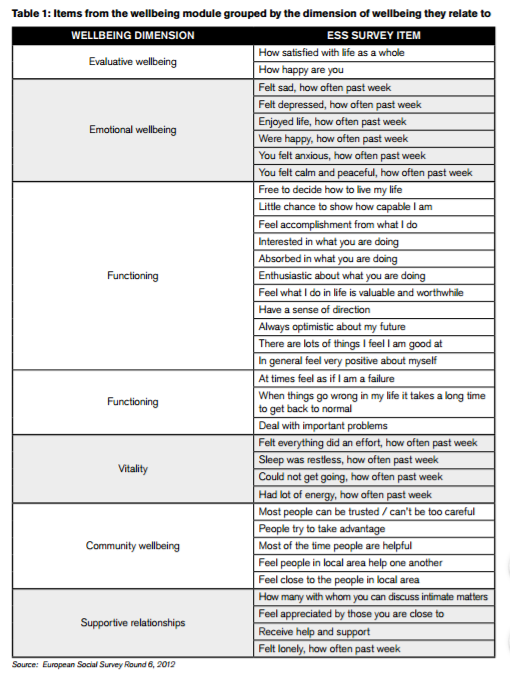
\includegraphics[scale=1]{surveyTable.png}
%\caption{\hl{Make a new table here}}
%\label{surveyTable}
%\end{figure}

%\begin{table}[t]
%\centering
%\begin{tabular}{cl}
%Wellbeing dimension & ESS item \\
%\multirow{2}{*}{Evaluative wellbeing} & X \\ & Y \\ 
%\end{tabular}
%\end{table}

\begin{table}[t]
\centering
\begin{tabular}{lccccccccc}
  \hline
  & \multicolumn{3}{c}{Denmark} & \multicolumn{3}{c}{Bulgaria} & \multicolumn{3}{c}{Sweden} \\
 & $Q_1$ & $M$ & $Q_3$ \quad & $Q_1$ & $M$ & $Q_3$ \quad & $Q_1$ & $M$ & $Q_3$ \\ 
  \hline
 Evaluative wellbeing & 8.00 & 8.75 & 9.50 & 3.50 & 5.00 & 7.00 & 7.00 & 8.00 & 9.00 \\ 
 Emotional wellbeing & 7.22 & 8.33 & 8.89 & 5.00 & 6.67 & 7.78 & 6.67 & 7.78 & 8.89 \\ 
Functioning & 6.93 & 7.57 & 8.21 & 5.50 & 6.68 & 7.68 & 6.39 & 7.04 & 7.68 \\ 
Vitality & 6.67 & 7.50 & 8.33 & 5.83 & 7.50 & 8.33 & 6.67 & 7.50 & 9.17 \\ 
 Community wellbeing & 5.83 & 6.77 & 7.57 & 3.70 & 4.67 & 5.70 & 5.66 & 6.57 & 7.37 \\ 
Supportive relationships & 7.42 & 8.25 & 8.92 & 6.17 & 7.25 & 8.08 & 7.42 & 8.25 & 8.75 \\ 
   \hline
\end{tabular}
\caption{The 1st quartile, the median and the third quartile of the distrubutions of each of the six dimensions of psychological well-being, stratified by country. Note that the scales are constructed such that they all run from 0-10.}
\label{tableDistr}
\end{table}


The ESS 2012 data contains a total of 626 variables collected from 54673 citizens in 29 countries. Here, we will only work with a subset of 35 questionnaire items that are all related to psychological well-being. These 35 items can be divided into 6 distinct scales, namely \textit{Evaluative wellbeing}, \textit{Emotional wellbeing}, \textit{Functioning}, \textit{Vitality}, \textit{Community wellbeing} and \textit{Supportive relationships}. More details on these scales is to be found in (\hl{ref: ESS6 Topline Results Series 5}). We represent each of these scales by a single variable, which is calculated as the average score within the items related to that variable (\hl{ref to someone that says that is sensible?}) and scaled such that it takes a value between 0 and 10. For simplicity, we use only complete cases for this construction and thus exclude all participants that did not answer all the 35 questionnaire items used below. This gives us $n_{DK} = 1498$ observations in the Danish sample, $n_{BG} = 1798$ observations in the Bulgarian sample and $n_{SE} = 1736$. Table \ref{tableDistr} summarizes the marginal distributions of the six dimensions of psychological well-being, stratified by country. 



\subsection{Comparing Denmark and Bulgaria}
\begin{figure}
\center
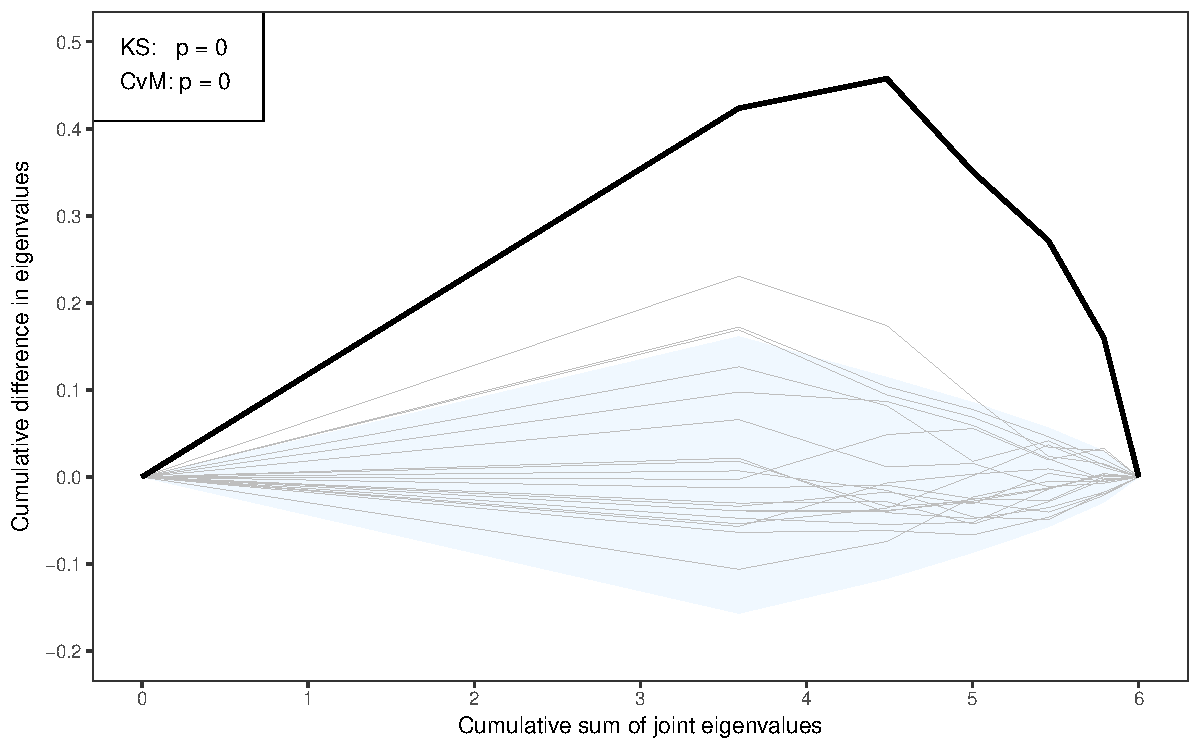
\includegraphics[scale = 0.7]{essDKBGce.pdf}
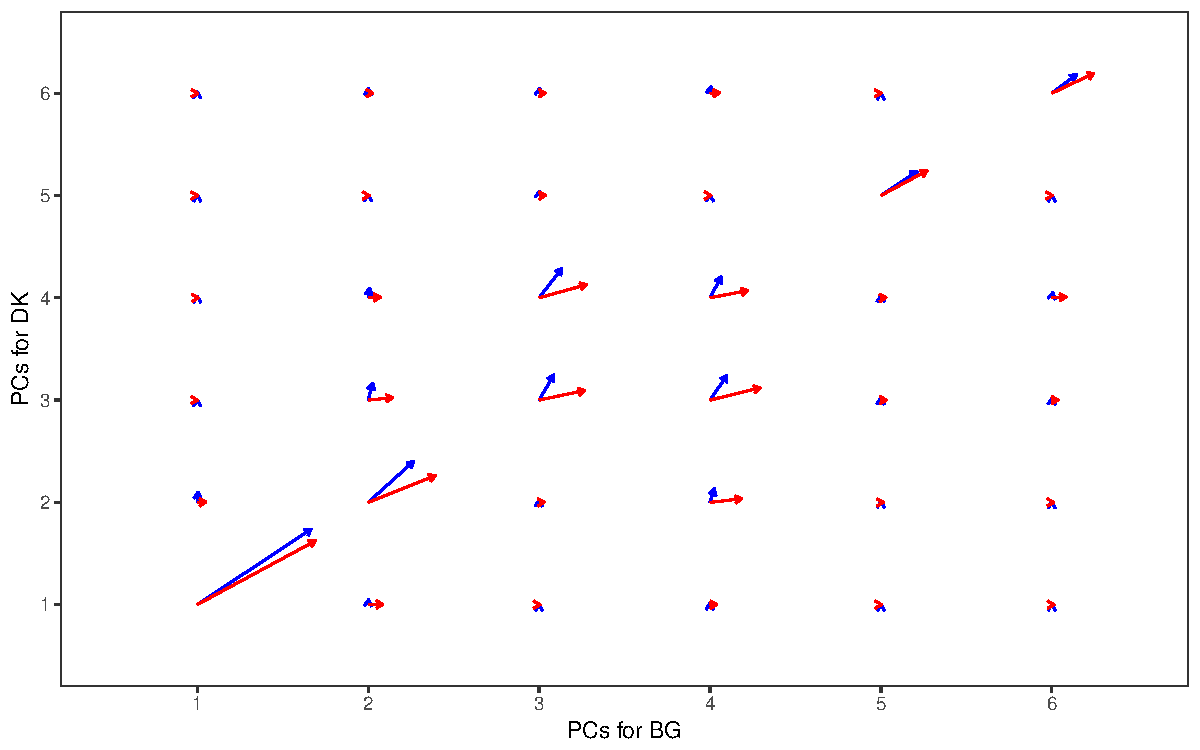
\includegraphics[scale = 0.7]{essDKBGhair.pdf}
\caption{The CE plot (top) and the angle plot (bottom) resulting from comparing Bulgarian and Danish data on psychosocial well-being. Dataset 1 refers to the Bulgarian subsample, while Dataset 2 is the Danish data. The CE plot is annotated with the $p$-values of the Kolmogorov-Smirnov and the Cram\'er-von Mises tests of the assumption of no difference in data structures. In the angle plot, the blue arrows show the principal components of the Bulgarian dataset decomposed in the coordinate system of the principal components of the Danish dataset, while the red arrows illustrate the reverse.}
\label{plotBG.cehair}
\end{figure}

\begin{figure}
\center
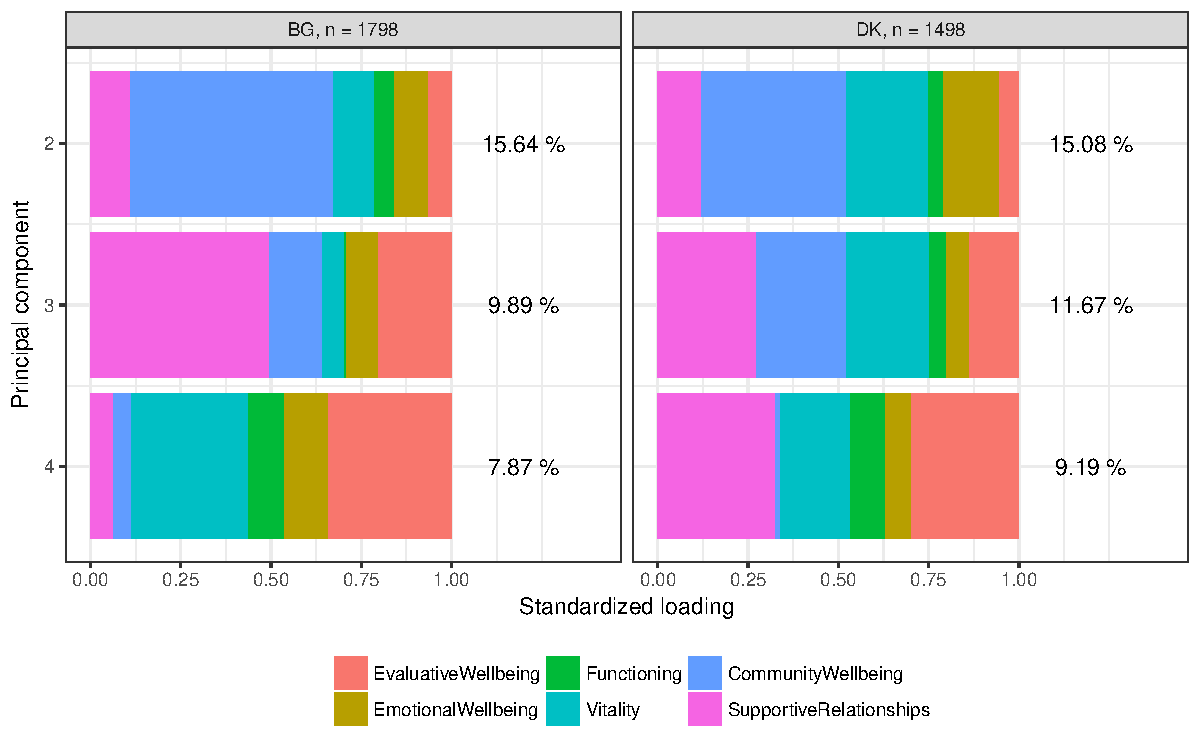
\includegraphics[scale = 0.7]{essDKBGpancake234.pdf}
\caption{\hl{something}}
\label{plotBG.pancake}
\end{figure}

%\begin{figure}
%\center
%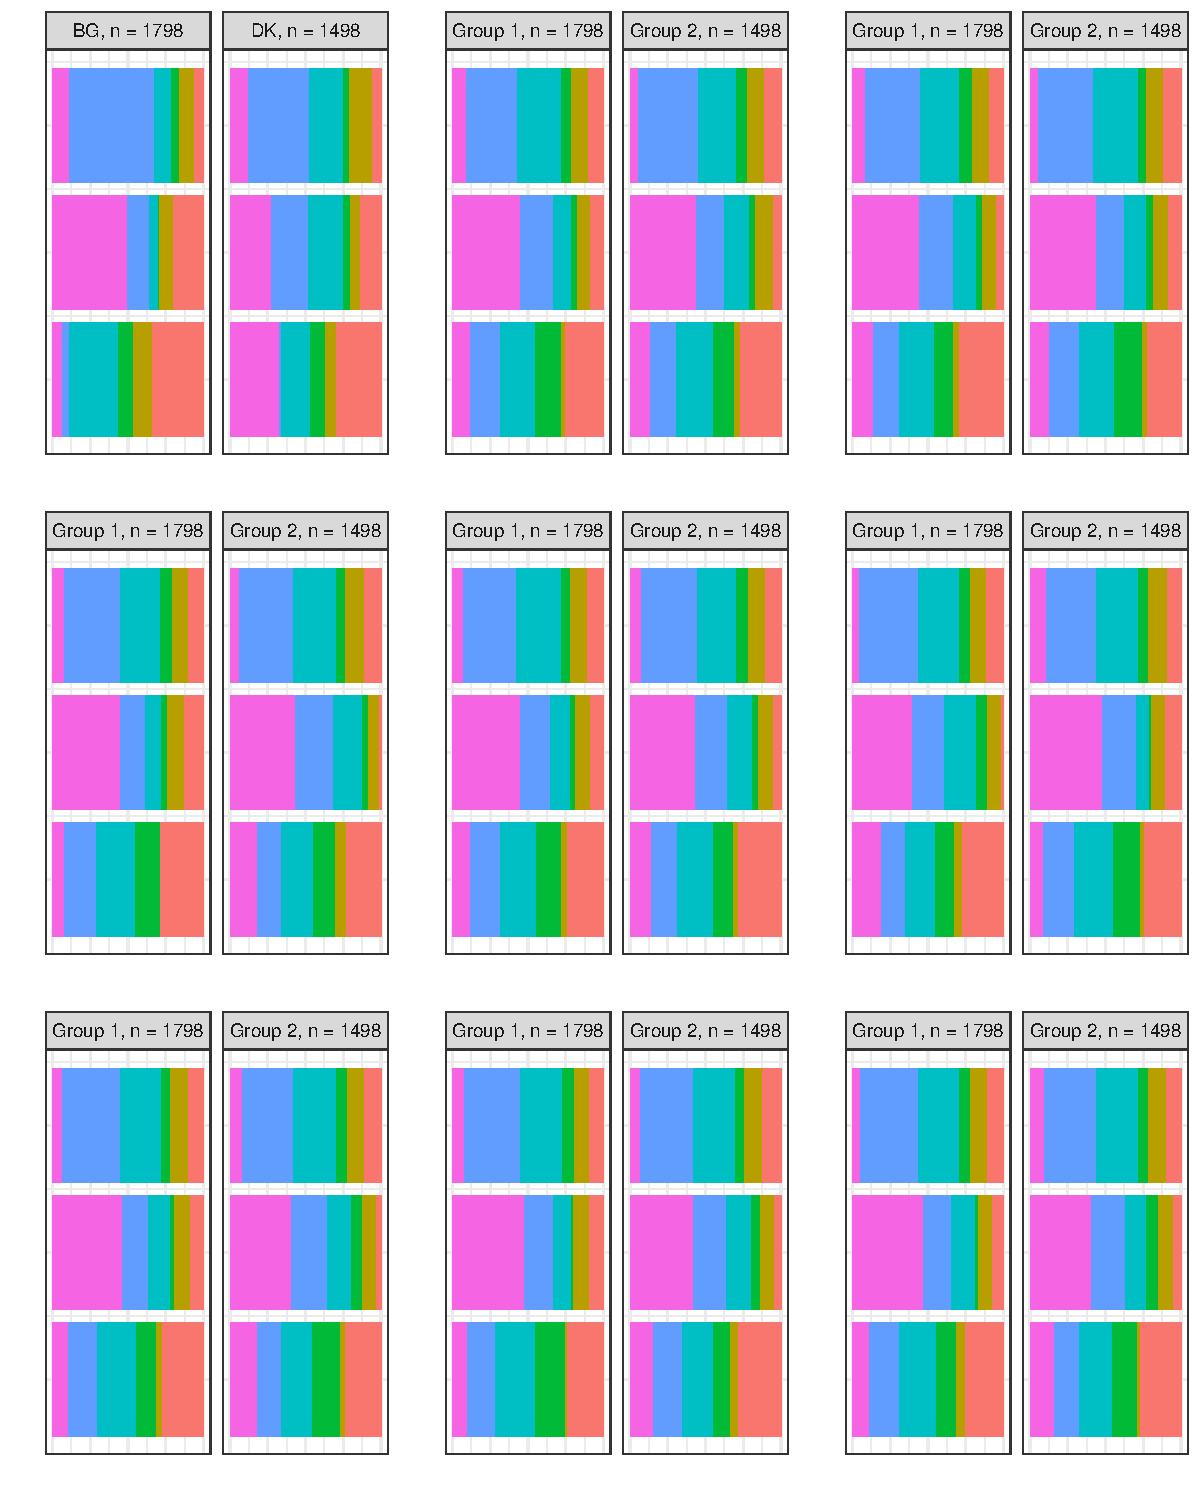
\includegraphics[scale = 0.7]{essDKBGWallyPCADSC234.pdf}
%\caption{\hl{something.}}
%\label{plotBG.wally}
%\end{figure}



Figure \ref{plotBG.cehair} presents the CE plot and the angle plot obtained from comparing the Danish and Bulgarian psychological well-being scales. The CE plot show a remarkable degree of lacking comparability: The cumulative difference in the eigenvalue by far exceeds what could come about randomly if there really was no difference in the data structure. This is also confirmed by the Kolmogorov-Smirnov and the Cram\'er-von Mises tests, which both result in $p$-values that are virtually zero. 

Moving on to the angle plot, we find that the differences are primarily to be found in the second, third and fourth principal components (PCs): The blue arrows visualize the decomposition of the principal components for the first dataset in the coordinate system of the second dataset. We see that PC2 also loads on PC3, that PC3 also loads on PC4, and that PC4 also loads on PC2 and PC3. The red arrows visualize the decomposition of the principal components for the second dataset in the coordinate system of the first dataset. Here, we see that PC2 also loads on PC4, that PC3 also loads on PC2 and PC4, and that PC4 also loads on PC3. Thus, if we wish to understand why differences in the data structures occur, an inspection of the loadings of components 2, 3 and 4 might be informative.

 The chroma blot in Figure \ref{plotBG.pancake} allows us to look closer into these components. Here, we find that the relative importance of the \textit{Community wellbeing} and \textit{Supportive relationships} scales is much larger in the Bulgarian sample than in the Danish. In the Danish data, on the other hand, we find that \textit{Vitality} and \textit{Emotional well-being} seem to play bigger roles, as they appear with larger loadings in more high-ranking components in this sample, relative to the Bulgarian. 
 
All in all, we find that psychological well-being does not seem to be the same concept in Bulgaria as in Denmark. The two countries disagree both in how many dimensions are needed to capture the most important parts of the concept (as illustrated by the differences in eigenvalue) and in how these dimensions are then weighted among the 6 scales (as illustrated by the angle and chroma plots). In Bulgaria, interpersonal features seem to be more informative of psychological wellbeing, whereas in Denmark, individual characteristic play a relatively bigger role. Thus, the datasets are fundamentally different and that we should therefore be wary about combining them in a joint analysis, which was also the conclusion of the ESS authors, though based on country-level aggregated statistics. \\

\hl{I have dropped the Wally-plots for now, as I'm not really sure they are that useful.}


% While the first principal component, which is responsible for explaining 50-60 \% of the variance in the data, is very similar for the two countries, we see quite large differences in the remaining components. In the second component, we see that the two countries disagree in the relative importance of the scales \textit{Community wellbeing} and \textit{Vitality}. In the third and fourth components, general disagreement  is found. All in all, components 2-4, representing almost half of the variability in the data, are not very similar across the two countries. Moreover, the two subsets of the data also differ with respect to how much variance is explained by each component, and the difference is particularly big for the first component. This component has approximately 15 \%  more explanatory power in the Bulgarian subsample than it does in the Danish.

%{\color{red}
%Figure \ref{plotESSHairplot} shows the hairplot. The blue arrows visualize the decomposition of the principal components for the %first dataset in the coordinate system of the second dataset. We see that PC2 also loads on PC3, that PC3 also loads on PC4, and %that PC4 also loads on PC2 and PC3. The red arrows visualize the decomposition of the principal components for the second dataset %in the coordinate system of the first dataset. We see that PC2 also loads on PC4, that PC3 also loads on PC2 and PC4, and that %PC4 also loads on PC3. For PC1, PC5 and PC6 the main difference is in the size of the variation component.
%}


%But did we really illustrate a data structure difference due to country differences or did we just illustrate the variability of the results of the PCADSC method? In order to investigate this further, we look at a so-called \textit{Wally plot} (\hl{ref: Claus Ekstrøm}). In this plot, we compare the results of PCADSC conducted with grouping by country with several random, but similar grouping variables. Specifically, we produce 7 PCADSC plots where the country variable was replaced by a randomly generated variable that divides the observations into two groups of the same sizes as the country samples. The results are illustrated in Figure \ref{plotESSPCADSCWally}. Here, we see that the differences in the second component from the original PCADSC results are not matched in any of the randomly grouped PCADSC runs. In fact, the 7 runs are remarkably similar, thereby illustrating that PCADSC seems to be very robust with respect to random groupings: The signal in the data is not blurred by the random subdivisions. When it comes to the differences in the third component for the two groups, we find much larger variability in the 7 random runs. \hl{more comments here... Wait until we are sure exactly what we think about the results and what other PCA-based methods, we will do before/after. Particularly, how do we deal with eigen value differences?}

\subsection{Comparing Denmark and Sweden}
\begin{figure}
\center
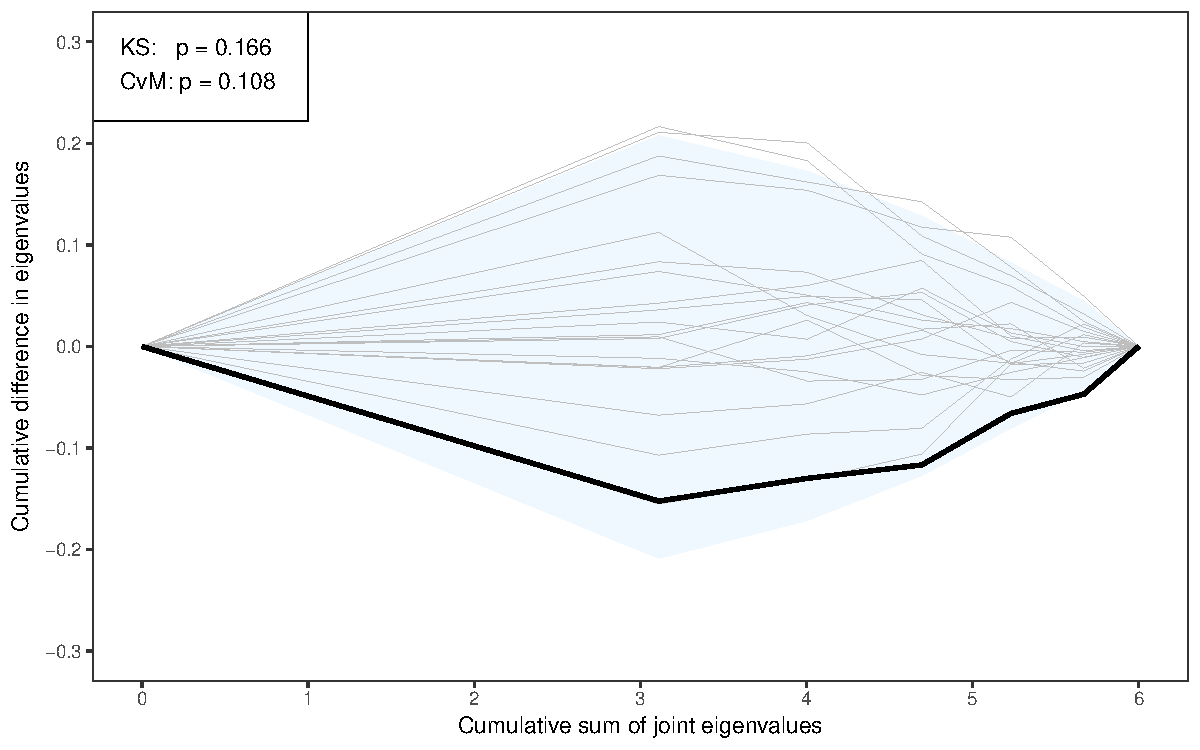
\includegraphics[scale = 0.7]{essDKSEce.pdf}
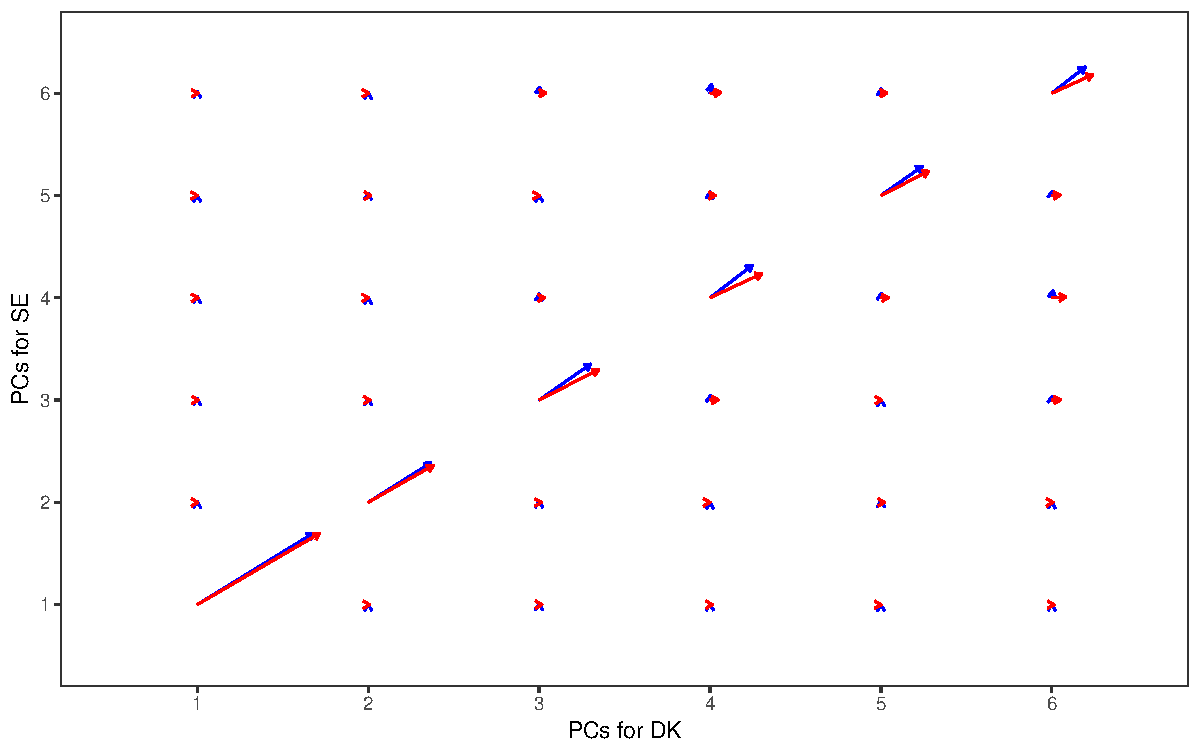
\includegraphics[scale = 0.7]{essDKSEhair.pdf}
\caption{A CE (top) and a hair (bottom) plot for comparing the Danish (Dataset 1) and the Swedish (Dataset 2) psychological well-being data. The blue arrows show the principal components of the Danish dataset decomposed in the coordinate system of the principal components of the Swedish dataset, and the red arrows illustrate the reverse.}
\label{plotSE.cehair}
\end{figure}

\begin{figure}
\center
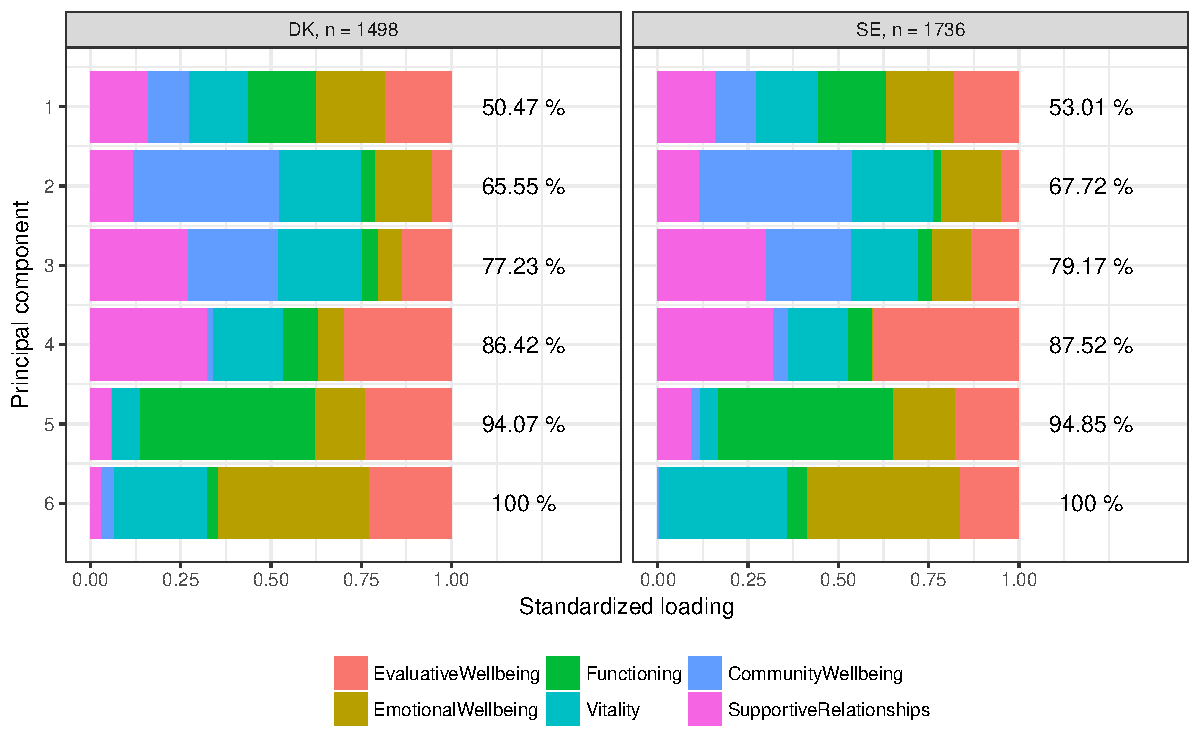
\includegraphics[scale = 0.7]{essDKSEpancake.pdf}
\caption{A chroma plot for comparing the loading patterns of the Danish and the Swedish subsamples. Note that the bars for each component is annotated with its cumulative variance score, that is, how much variance can be explained by having information of this and the preceding components.}
\label{plotSE.pancake}
\end{figure}

%\begin{figure}
%\center
%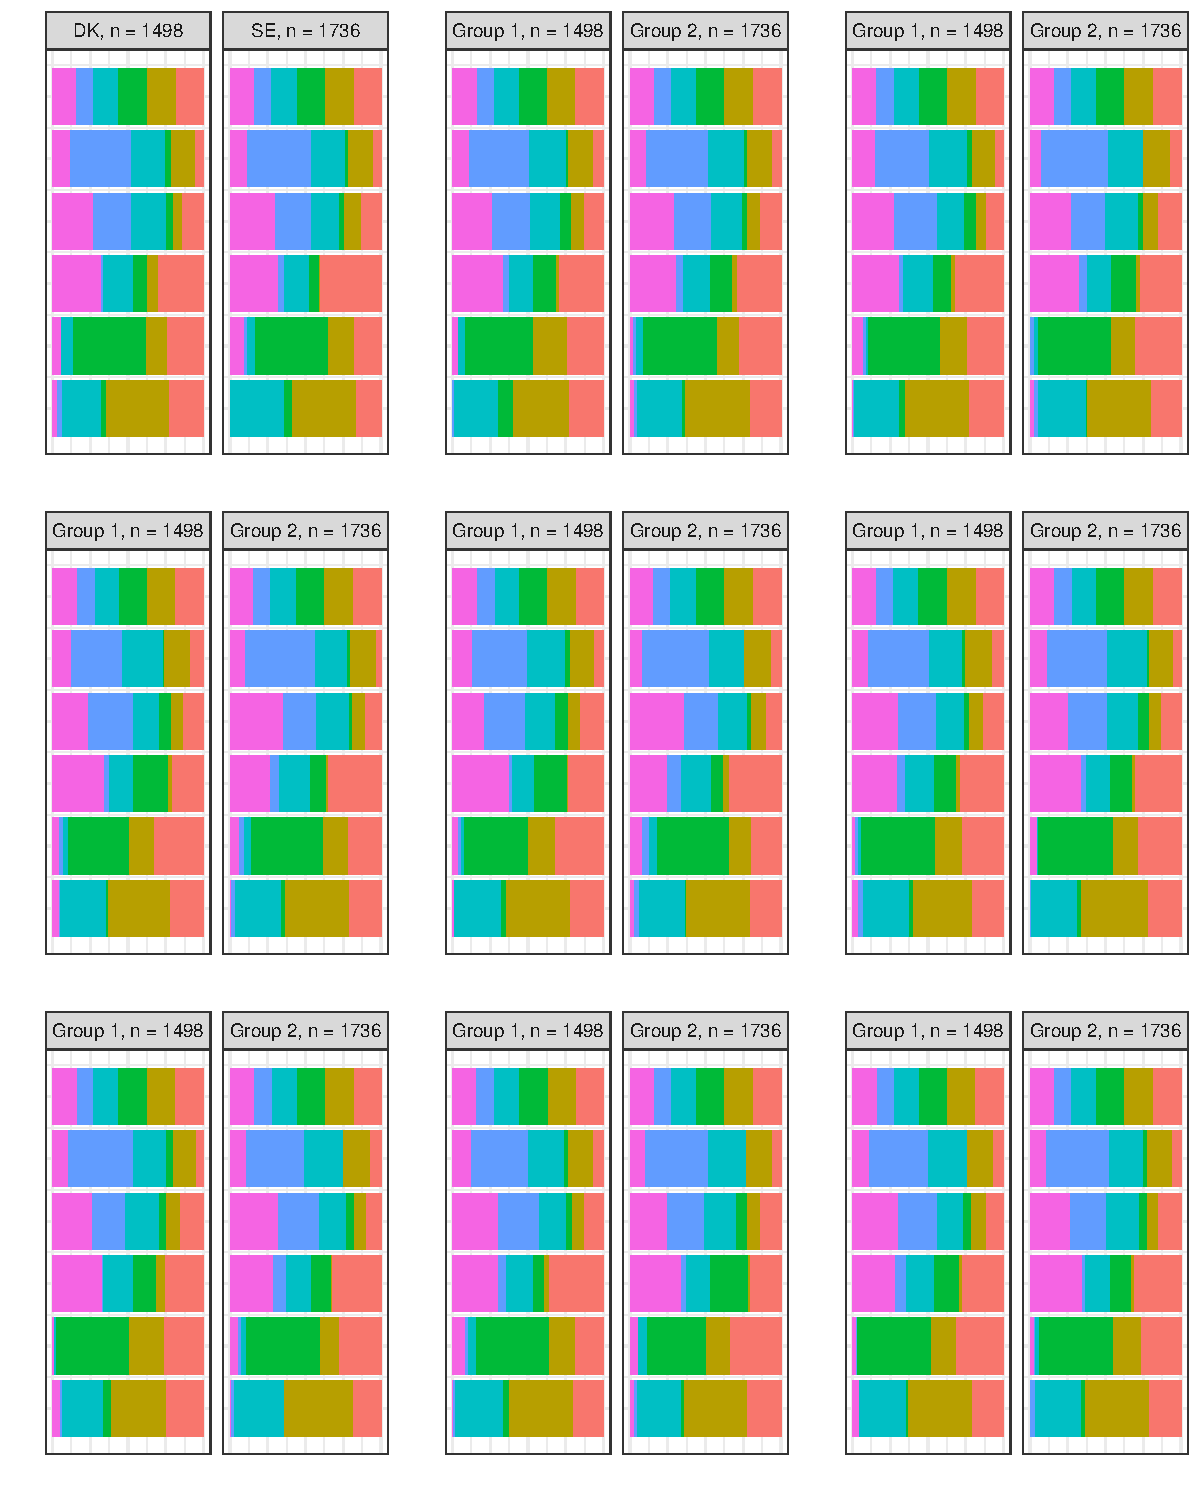
\includegraphics[scale = 0.7]{essDKSEWallyPCADSC.pdf}
%\caption{\hl{something.}}
%\label{plotSE.wally}
%\end{figure}

We now turn to the comparison of Denmark and Sweden in terms of psychological well-being. Figure \ref{plotSE.cehair} show the CE and angle plots for these two countries. In the CE plot, we now find the cumulative eigenvalue curve to be just within the acceptance region of the null-hypothesis. This is also reflected by the two tests, which now produce $p$-values of $p_{KS} = 0.14$ and $p_{CvM} = 0.09$, respectively, thus accepting the null-hypothesis at the typical 5\% level, but not with overwhelming evidence. 

The angle plot from Figure \ref{plotSE.cehair} shows that the two datasets agree very strongly about the relative importance of the six scales in the six PCs, as almost all off-diagonal arrows are practically non-existent. This implies that if one already has e.g. the information held in the first PC from the Danish data, this information is in itself mostly sufficient to describe the first PC of the Swedish data. 

Looking at the chroma plot in Figure \ref{plotSE.pancake}, the same tale is told once again: Here, we find remarkably similar loading patterns in the first three components (which are responsible for almost 80 \% of the variance in both datasets), and slight, but increasing, differences in the remaining three components. We therefore conclude that any differences in the data structures of the Danish and the Swedish samples are related to the least important dimensions of the datasets and that these dimensions are only responsible for less than 25 \% of the variance in both datasets. In particular, this means that we can combine and compare the Danish and Swedish datasets in a meaningful way and e.g. conclude using Table \ref{tableDistr} that in general, Danes seem to be somewhat more happy than Swedes, and in particular, the unhappy people in Denmark (represented by the 1st quartiles) are generally a lot happier in Denmark than they are in Sweden. A more thorough, statistical investigation could now be put to work on answering \textit{why} this seems to be the case. 

\section{Discussion}
\label{sec:discussion}
\hl{
\begin{itemize}
\item Generalizing the results to non-numeric variables?
	\begin{itemize}
		\item Interpretation for binary variables?
		\item Any meaningful way to allow for nominal, categorical variables?
		\item ... ?
	\end{itemize}
\item Generalizing the results to covariance matrices that are not of full rank?
\item Investigate sensitivity towards the sample sizes $n_1$ and $n_2$
\item Limitations: What sorts of problems can never be found using PCADSC? 
\begin{itemize}
\item Differences in scaling, as we standardize all variables
\item More?
\end{itemize}
\end{itemize}
}

%\section{Concluding Remarks}
%\label{sec:conclusion}

\vspace{\fill}\clearpage
\newpage
\bibliographystyle{apa}
\bibliography{bib}

\end{document}
